\section{Darstellung der Ergebnisse und Auswertung}

\subsection{Darstellung der Ergebnisse}
Mit der oben beschriebenen Messmethode, wurden folgende Werte gemessen:
\begin{table}

\begin{tabular}{|c|c|}
\hline 
t in s & dN/dt in 1/10s \\ 
\hline
20	&34\\ 
\hline
40	&29\\ 
\hline
60	&32\\ 
\hline
80	&28\\ 
\hline
100	&31\\ 
\hline
120	&25\\ 
\hline
140	&28\\ 
\hline
160	&24\\ 
\hline
180	&27\\ 
\hline
200	&24\\ 
\hline
220	&32\\ 
\hline
240	&25\\ 
\hline
260	&24\\ 
\hline
280	&27\\ 
\hline	
300	&26\\ 
\hline
320	&25\\ 
\hline
340	&27\\ 
\hline
420	&29\\ 
\hline	
440	&29\\ 
\hline
460	&26\\ 
\hline
480	&25\\ 
\hline
500	&26\\ 
\hline
560	&26\\ 
\hline
580	&22\\ 
\hline	
600	&25\\ 
\hline
620	&22\\ 
\hline
640	&21\\ 
\hline
660	&20\\ 
\hline
680	&23\\ 
\hline
700	&21\\ 
\hline
760	&22\\ 
\hline
780	&20\\ 
\hline
800	&24\\ 
\hline
820	&22\\ 
\hline
840	&24\\ 
\hline
860	&23\\ 
\hline
880	&22\\ 
\hline
900	&20\\ 
\hline
920	&22\\ 
\hline
940	&20\\ 
\hline
960	&21\\ 
\hline
980	&22\\ 
\hline
1000&	18\\ 
\hline
1080&	19\\ 
\hline	
1100&	19\\ 
\hline
1120&	18\\ 
\hline
1160&	17\\ 
\hline
1180&	16\\ 
\hline
1200&	18\\ 
\hline
1220&	18\\ 
\hline
1240&	16	\\ 
\hline
1260&	17\\ 
\hline
1280&	15\\ 
\hline
1300&	18\\ 
\hline
1320&	16\\ 
\hline
1340&	15\\ 
\hline
1360&	14\\ 
\hline
1440&	13\\ 
\hline
1460&	12\\ 
\hline
1480&	12	\\ 
\hline
1500&	13\\ 
\hline
1520&	12\\ 
\hline
1540&	12\\ 
\hline
1560&	10	\\ 
\hline
1580&	12\\ 
\hline
1600&	12\\ 
\hline
1640&	9\\ 
\hline
1660&	8\\ 
\hline
1680&	8\\ 
\hline
1700&	8\\ 
\hline
1720&	9\\ 
\hline
1740&	8\\ 
\hline
1760&	8\\ 
\hline
1780&	8\\ 
\hline
1840&	7\\ 
\hline
1860&	6\\ 
\hline
1880&	7\\ 
\hline
1900&	6\\ 
\hline
1920&	6\\ 
\hline
1940&	6\\ 
\hline
2000&	5\\ 
\hline
2020&	5\\ 
\hline
2040&	5\\ 
\hline
2060&	5\\ 
\hline
2080&	5\\ 
\hline
2160&	5\\ 
\hline
2180&	4\\ 
\hline
2200&	4\\ 
\hline
2220&	3\\ 
\hline
\end{tabular} 

\label{tbl_1}
\caption{Anzahl der innerhalb von 10s durchgelaufenen Ringe in Abhängigkeit der Zeit}
\end{table}

\begin{comment}

\begin{figure}
        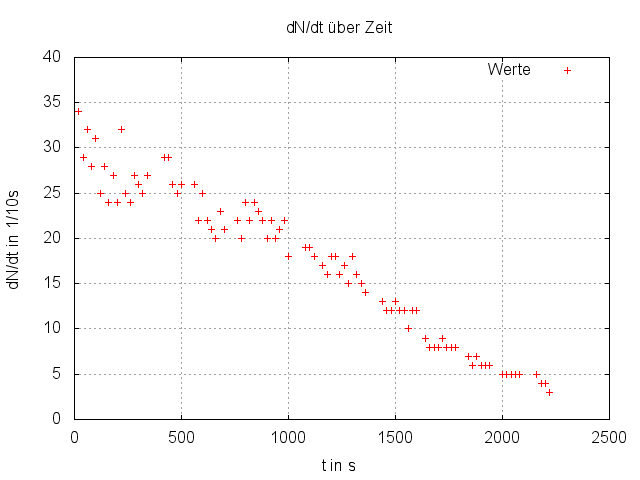
\includegraphics[width=.9\textwidth]{images/dNdt(t).png}
\caption{Anzahl der innerhalb von 10s druchgelaufenen Ringe in Abhängigkeit der Zeit}
\label{dNdt(t)}
\end{figure}


\end{comment}

Beim Betrachten von \ref{dNdt(t)} fällt sofort auf, dass die Messwerte bei großen Werten von dN/dt wesentlich mehr streuen, was darauf zurückzuführen ist, dass das Zählen der Ringe bei größeren Werten von dN/dt mehr Schwierigkeiten bereitet hat.
Eine Tabelle der Temperatur des Stabes in Abhängigkeit der Zeit ist im Anhang zu finden. \\
\ref{T(t)}

\begin{comment}

\begin{figure}
	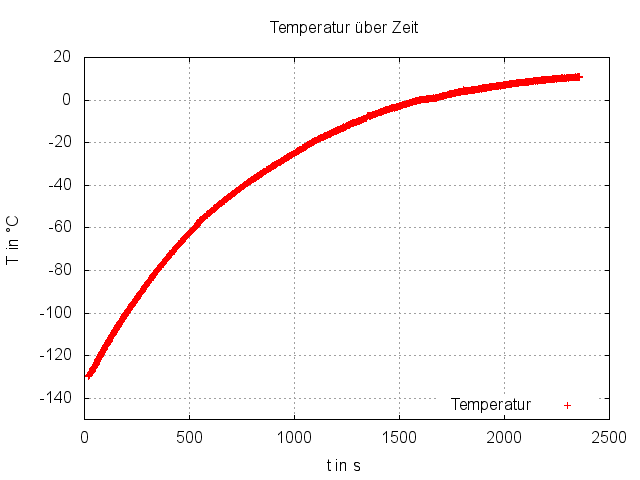
\includegraphics[width=.9\textwidth]{images/T(t).png}
\label{T(t)}
\caption{Temperatur in Abhängigkeit der Zeit}
\end{figure}

\end{comment}

An der Temperaturkurve ist bei $ 0 ^{\circ} C $ ein kurzes Gleichbleiben der Temperatur zu beobachten. Dies ist darauf zurückzuführen, dass sich Eis um den Stab gebildet hat. Dieses schmilzt bei $ 0 ^{\circ} C $ und hält den Stab so kurzzeitig auf einer konstanten Temperatur.

\subsection{Auswertung}
Aus den gemessenen Daten kann der Wärmeausdehnungskoeffizient $ \alpha $ des verwendeten Stabes in Abhängigkeit von der Temperatur bestimmt werden. Dafür werden in dieser Auswertung zwei verschiedene Methoden verwendet und anschließend miteinander verglichen.

\subsubsection{Einteilung der Messwerte in Fraktionen}
Bei dieser Methode werden die Messwerte möglichst gleichmäßig in Fraktionen eingeteilt und jeweils innerhalb dieser der Mittelwert von dN/dt gebildet.\\(Die Mittelwertbildung ist aus mehreren Gründen gerechtfertigt: Zum Einen wird gerade ein gemittelter Wärmeausdehnungskoeffizient bestimmt. Zum anderen kann dN/dt in den Fraktionen als linear approximiert werden, wodurch sich Abweichungen vom Mittelwert durch die Linearität gegenseitig aufheben.) Außerdem werden aus den zu den Fraktionen passenden Zeitintervallen die entsprechenden Zeitdifferenzen errechnet. Aus den so bestimmten Größen kann dann für jede Fraktion ein mittlerer Wärmeausdehnungskoeffizient folgendermaßen ermittelt werden:

\begin{equation}
\alpha(T)=\frac{\Delta L(T)}{L_{0}} \cdot \Delta T
\end{equation}

Aus $ \Delta L = \frac{\lambda}{2} \cdot \Delta N $ folgt:

\begin{equation}
\alpha (T)= \frac{\lambda}{2} \cdot \frac{\Delta N(T)}{L_0} \cdot \Delta T
\end{equation}

\begin{table}
\begin{tabular}{|c|c|c|}
\hline
Fraktion&	Zeitintervalle in s	& $\Delta T $ in $ ^{\circ} C$ \\
\hline
1		&[20, 180]		&26,5\\
\hline
2		&[200, 340]		&18,9\\
\hline
3		&[420, 500]		&8,7\\
\hline
4		&[560, 700]		&11,1\\
\hline
5		&[760, 880]		&7,9\\
\hline
6		&[900,1000]		&6,1\\
\hline
7		&[1080,1120]		&1,9\\
\hline
8		&[1160,1260]		&4,4\\
\hline
9		&[1280,1360]		&3,6\\
\hline
10		&[1440,1600]		&4,6\\
\hline
11		&[1640,1780]		&2,9\\
\hline
12		&[1840,1940]		&1,8\\
\hline
13		&[2000,2080]		&1,3\\
\hline
14		&[2160,2220]		&0,7\\
\hline
\end{tabular}

\caption{Einteilung in Fraktionen}
\label{tbl_2}
\end{table}



Innerhalb dieser Fraktionen ergeben sich folgende Mittelwerte mit zugehörigen Fehlern:

\begin{table}
\begin{tabular}{|c|c|c|}

\hline
Fraktion	&Mittelwert von dN/dt in 1/10s	&Fehler von dN/dt in 1/10s \\
\hline
1		&28,67				&1,08\\
\hline
2		&26,25				&0,92\\
\hline
3		&27					&0,84\\
\hline
4		&22,5				&0,73\\
\hline
5		&22,43				&0,53\\
\hline
6		&20,5				&0,62\\
\hline
7		&18,67				&0,33\\
\hline
8		&17					&0,37\\
\hline
9		&15,6				&0,68\\
\hline
10		&12					&0,29\\
\hline
11		&8,25				&0,16\\
\hline
12		&6,33				&0,21\\
\hline
13		&5					&0\\
\hline
14		&4					&0,41\\
\hline
\end{tabular}
\caption{Mittelwerte und Fehler von dN/dt}
\label{tbl_3}
\end{table}


An Tabelle \ref{tbl_3} fällt sofort auf, dass der Fehler in Fraktion 13 Null ist. Dies resultiert daraus, dass alle in dieser Fraktion zusammengefassten Werte gleich 5/10s sind.


\begin{comment}

\begin{figure}
        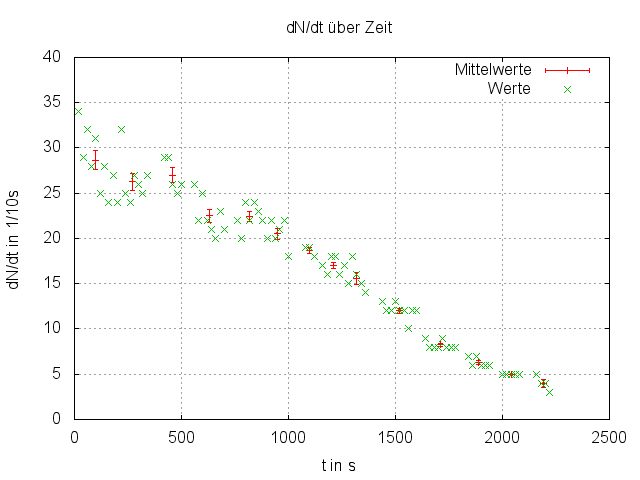
\includegraphics[width=.9\textwidth]{images/dNdt(t)MWmitaltenWerten.png}
\caption{Einteilung in Fraktionen}
\label{dNdt(t)MWmitaltenWerten}
\end{figure}

\end{comment}

\ref{dNdt(t)MWmitaltenWerten}

Für die Fehlerabschätzung von $ \alpha $ wird eine Fehlerfortpflanzung durchgeführt.
Dabei sind die Fehler von $ \lambda $  und  $ \Delta T $ vernachlässigbar klein. Im Fall von $ \Delta T $ ist der Fehler sogar nicht ermittelbar, da auf Grund der Benutzung von CASSY diesbezüglich keine ausreichenden Angaben vorhanden sind.

Der Fehler von $ L_{0} $ ist laut Versuchsaufbau $ 1 mm $.

Die Fehlerfortpflanzung liefert:

\begin{equation}
\Delta (\alpha) = \frac{\lambda}{2 \cdot \Delta T} \cdot \sqrt{\frac{1}{L_{0}^{2}} \cdot (\Delta(\Delta N))^{2} + \frac{(\Delta N)^{2}}{(L_{0})^{4}} \cdot (\Delta L_{0})^{2}}
\end{equation}


Es ergibt sich so:

\begin{table}
\begin{tabular}{|c|c|c|}
\hline
Mittlere Temperatur in $^{\circ}C$ &$ \alpha $ in $ 10^{-5}\frac {1}{^{\circ}C} $	&Fehler von $ \alpha $ in $ 10^{-5} \frac{1}{^{\circ}C}  $ \\
\hline
-115,6&				1,896	&		0,072\\
\hline
-90,2	&			2,129	&		0,075\\
\hline
-66,9	&			2,719	&		0,085\\
\hline
-50,1	&			3,108	&		0,101\\
\hline
-35,9	&			3,731	&		0,089\\
\hline
-27,9	&			3,680	&		0,112\\
\hline
-19,2	&			4,305	&		0,078\\
\hline
-14,0	&			4,231	&		0,093\\
\hline
-9,3	&			3,797	&		0,166\\
\hline
-2,1	&			4,571	&		0,112\\
\hline
2,1		&		4,362		&	0,086\\
\hline
5,3		&		3,851		&	0,128\\
\hline
7,7		&		3,370		&	0,011\\
\hline
9,4		&		3,755		&	0,385\\
\hline
\end{tabular}
\label{tbl_4}
\caption{Wärmeausdehnungskoeffizient in Abhängigkeit der Temperatur}
\end{table}

\begin{comment}

\begin{figure}
        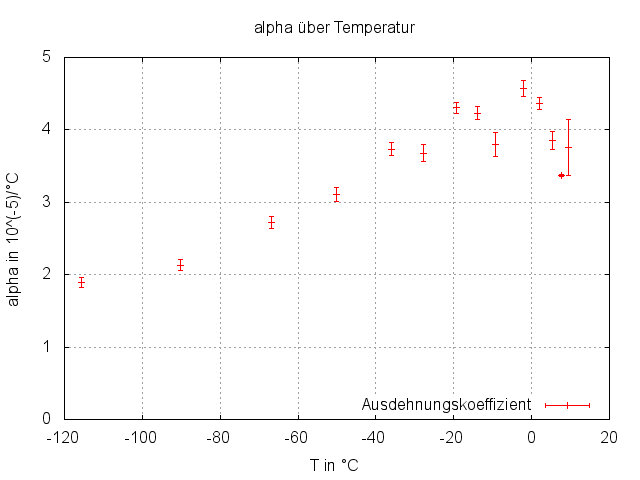
\includegraphics[width=.9\textwidth]{images/alpha(T).png}
\caption{Wärmeausdehnungskoeffizient in Abhängigkeit der Temperatur}
\label{alpha(T)}
\end{figure}

\end{comment}


\subsubsection{Berechnung des Ausdehnungskoeffizienten durch approximatives Fitten}

Bei dieser Methode werden dN/dt und T(t) gefittet und daraus der Ausdehnungskoeffizient in Abhängigkeit der Temperatur bestimmt.

dN/dt lässt sich gut mit einem Polynom 5. Grades approximieren:

\begin{equation}
 N^{*} := dN/dt 
\end{equation}

Dabei ergibt sich für 


\begin{equation}
N^{*}(t)=a_{0}+a_{1} \cdot t+a_{2}t^{2}+a_{3}t^{3}+a_{4}t^{4}+a_{5}t^{5} :
\end{equation}

$
 a_{0} =(3,153 \pm 0,104) s^{-1} 
$

$
a_{1}=(-0,00311 \pm 0,00097)s^{-2}
$

$
a_{2}=(5,78 \pm 2,65)10^{-6}s^{-3}
$

$
a_{3}=(-5,83 \pm 2,99)10^{-9}s^{-4}
$

$
a_{4}=(2,33 \pm 1,47)10^{-12}s^{-5}
$

$
a_{5}=(-3,21 \pm 2,62)10^{-16}s^{-6} 
$\\


\begin{comment}

\begin{figure}
        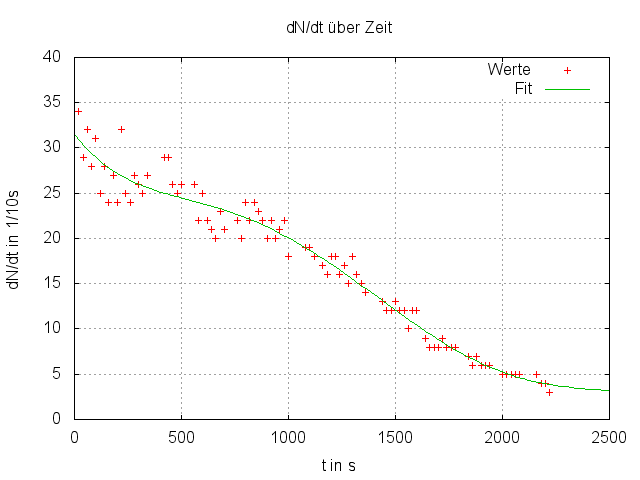
\includegraphics[width=.9\textwidth]{images/Fit dNdt(t).png}
\caption{Fit von dN/dt}
\label{Fit dNdt(t)}
\end{figure}

\end{comment}

T(t) lässt sich sehr gut mit einer e-Funktion approximieren:

Dabei ergibt sich für $ T(t) = a \cdot e^{bt} + c $ :

$a = (-154,01 \pm 0,04)^{\circ}C$,
$b=(-0,0012499 \pm 0,0000011)s^{-1}$,
$c=(19,91 \pm 0,042)^{\circ}C$

\begin{comment}

\begin{figure}
        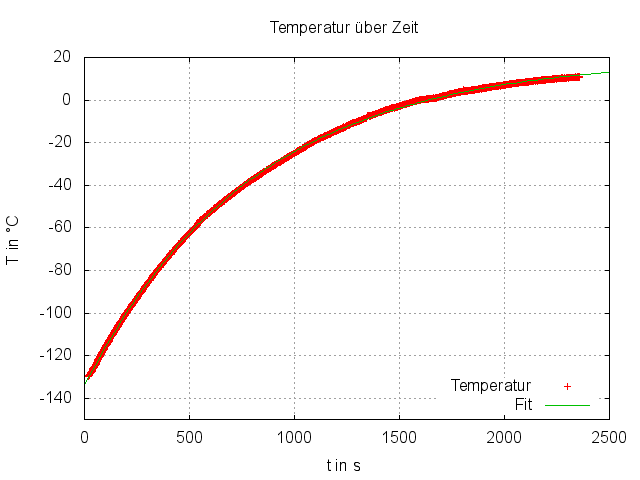
\includegraphics[width=.9\textwidth]{images/Fit T(t).png}
\caption{Fit von T(t)}
\label{Fit T(t)}
\end{figure}

\end{comment}

Herleitung einer Formel zur Berechnung des Ausdehnungskoeffizienten:

Wegen $ \Delta L = \alpha \cdot L_{0} \cdot \Delta T $ folgt: 
\\
\begin{equation}
\alpha (T) = \frac{1}{L_{0}} \frac{\partial L}{\partial T}
\end{equation}
Außerdem gilt: 
\begin{equation}
L = \frac{\lambda}{2} N
\end{equation}

\begin{equation}
\Rightarrow \alpha(T) = \frac{1}{L_{0}} \frac{\lambda}{2} \frac{\partial N}{\partial T} = \frac{\lambda}{2} \cdot L_{0} \frac{\partial N}{\partial t} \frac{\partial t}{\partial T}
\end{equation}

\begin{equation}
\Rightarrow \alpha (T) = \frac{\lambda}{2 \cdot L_{0}} \frac{N^{\cdot}(t(T))}{T^{\cdot}(t(T))}
\end{equation} 
mit 

Dann ergibt sich folgender Graph:

\begin{comment}

\begin{figure}
        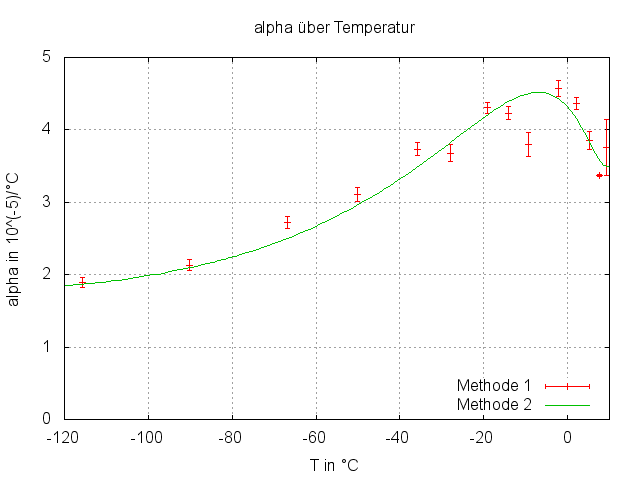
\includegraphics[width=.9\textwidth]{images/alpha(T)mitFit.png}
\caption{Vergleich zwischen Methode 1 und 2}
\label{alpha(T)mitFit}
\end{figure}

\end{comment}

Aus beiden Methoden lässt sich folgern, dass der mittlere Wärmeausdehnungkoeffizient des Stabs von der Temperatur abhängig ist.

\subsection{Fazit}


Der Bau des Interferometers hat sich als sehr schwierig herrausgestellt, da die Spiegel sehr genau ausgerichtet sein müssen.
Weitere Probleme sind bei der Messung der Ausdehnung des Stabs entstanden. Der vom Stab geschobene Spiegel musste so auf einer Schiene befestigt sein, dass er sich dabei nicht verdreht.
Durch das Zählen von Interferenzringen konnten dennoch Messungen durchgeführt werden, welche damit die Funktionstüchtigkeit des Michelson-Interferometers bestätigten.


